\documentclass[twoside]{article}

% Packages required by doxygen
\usepackage{fixltx2e}
\usepackage{calc}
\usepackage{doxygen}
\usepackage[export]{adjustbox} % also loads graphicx
\usepackage{graphicx}
\usepackage[utf8]{inputenc}
\usepackage{makeidx}
\usepackage{multicol}
\usepackage{multirow}
\PassOptionsToPackage{warn}{textcomp}
\usepackage{textcomp}
\usepackage[nointegrals]{wasysym}
\usepackage[table]{xcolor}

% Font selection
\usepackage[T1]{fontenc}
\usepackage[scaled=.90]{helvet}
\usepackage{courier}
\usepackage{amssymb}
\usepackage{sectsty}
\renewcommand{\familydefault}{\sfdefault}
\allsectionsfont{%
  \fontseries{bc}\selectfont%
  \color{darkgray}%
}
\renewcommand{\DoxyLabelFont}{%
  \fontseries{bc}\selectfont%
  \color{darkgray}%
}
\newcommand{\+}{\discretionary{\mbox{\scriptsize$\hookleftarrow$}}{}{}}

% Page & text layout
\usepackage{geometry}
\geometry{%
  a4paper,%
  top=2.5cm,%
  bottom=2.5cm,%
  left=2.5cm,%
  right=2.5cm%
}
\tolerance=750
\hfuzz=15pt
\hbadness=750
\setlength{\emergencystretch}{15pt}
\setlength{\parindent}{0cm}
\setlength{\parskip}{0.2cm}
\makeatletter
\renewcommand{\paragraph}{%
  \@startsection{paragraph}{4}{0ex}{-1.0ex}{1.0ex}{%
    \normalfont\normalsize\bfseries\SS@parafont%
  }%
}
\renewcommand{\subparagraph}{%
  \@startsection{subparagraph}{5}{0ex}{-1.0ex}{1.0ex}{%
    \normalfont\normalsize\bfseries\SS@subparafont%
  }%
}
\makeatother

% Headers & footers
\usepackage{fancyhdr}
\pagestyle{fancyplain}
\fancyhead[LE]{\fancyplain{}{\bfseries\thepage}}
\fancyhead[CE]{\fancyplain{}{}}
\fancyhead[RE]{\fancyplain{}{\bfseries\leftmark}}
\fancyhead[LO]{\fancyplain{}{\bfseries\rightmark}}
\fancyhead[CO]{\fancyplain{}{}}
\fancyhead[RO]{\fancyplain{}{\bfseries\thepage}}
\fancyfoot[LE]{\fancyplain{}{}}
\fancyfoot[CE]{\fancyplain{}{}}
\fancyfoot[RE]{\fancyplain{}{\bfseries\scriptsize Generated on Wed May 11 2016 16\+:14\+:44 for covafill by Doxygen }}
\fancyfoot[LO]{\fancyplain{}{\bfseries\scriptsize Generated on Wed May 11 2016 16\+:14\+:44 for covafill by Doxygen }}
\fancyfoot[CO]{\fancyplain{}{}}
\fancyfoot[RO]{\fancyplain{}{}}
\renewcommand{\footrulewidth}{0.4pt}
\renewcommand{\sectionmark}[1]{%
  \markright{\thesection\ #1}%
}

% Indices & bibliography
\usepackage{natbib}
\usepackage[titles]{tocloft}
\setcounter{tocdepth}{3}
\setcounter{secnumdepth}{5}
\makeindex

% Hyperlinks (required, but should be loaded last)
\usepackage{ifpdf}
\ifpdf
  \usepackage[pdftex,pagebackref=true]{hyperref}
\else
  \usepackage[ps2pdf,pagebackref=true]{hyperref}
\fi
\hypersetup{%
  colorlinks=true,%
  linkcolor=blue,%
  citecolor=blue,%
  unicode%
}

% Custom commands
\newcommand{\clearemptydoublepage}{%
  \newpage{\pagestyle{empty}\cleardoublepage}%
}


%===== C O N T E N T S =====

\begin{document}

% Titlepage & ToC
\hypersetup{pageanchor=false,
             bookmarks=true,
             bookmarksnumbered=true,
             pdfencoding=unicode
            }
\pagenumbering{roman}
\begin{titlepage}
\vspace*{7cm}
\begin{center}%
{\Large covafill \\[1ex]\large v0.\+2.\+3 }\\
\vspace*{1cm}
{\large Generated by Doxygen 1.8.9.1}\\
\vspace*{0.5cm}
{\small Wed May 11 2016 16:14:44}\\
\end{center}
\end{titlepage}
\tableofcontents
\pagenumbering{arabic}
\hypersetup{pageanchor=true}

%--- Begin generated contents ---
\section{Main Page}
\label{index}\hypertarget{index}{}covafill is a C++ template library for local polynomial regression of covariates in state-\/space models. The covafill library is based on the \href{http://http://eigen.tuxfamily.org}{\tt Eigen} library for linear algebra, and includes several modules\+:


\begin{DoxyItemize}
\item The \hyperlink{group__core}{Core module} which provides the base functionality for local polynomial regression
\item The \hyperlink{group__tree}{Tree module} which provides a search tree approximation to local polynomial regression
\item The \hyperlink{group__interpolate}{Interpolate module} which provides classes for cubic interpolation in 1-\/3 dimensions. This module is only inteded for internal use.
\item The \hyperlink{group__jags}{J\+A\+G\+S module}, which provides a module for using covafill with \href{http://mcmc-jags.sourceforge.net/}{\tt J\+A\+G\+S}
\item The \hyperlink{group__tmb}{T\+M\+B module} which provides functionality to use covafill with \href{http://tmb-project.org}{\tt T\+M\+B}.
\end{DoxyItemize}

\subsubsection*{The Core module}

The Core module provides the class \hyperlink{classcovafill}{covafill} for local polynomial regression.

\paragraph*{Local polynomial regression}

For simplicity, consider the univariate model

\[ y_i = g(x_i) + \epsilon_i \]

where $g:\mathbb{R}\mapsto\mathbb{R}$ is a smooth function and $ \epsilon_i\sim N(0,\sigma^2)$. To do local polynomial regression of $g$ at $x_0$, we do a Taylor expansion of order $p$,

\[ g(x) \approx g(x_0) + g^{(1)}(x_0)(x-x_0) + \frac{1}{2!} g^{(2)}(x_0)(x-x_0)^2 + \cdots + \frac{1}{p!} g^{(p)}(x_0)(x-x_0)^p \] Substituting into the original model, \[ y_i = g(x_0) + g^{(1)}(x_0)(x-x_0) + \frac{1}{2!} g^{(2)}(x_0)(x-x_0)^2 + \cdots + \frac{1}{p!} g^{(p)}(x_0)(x-x_0)^p + \epsilon_i \] we obtain a linear model with coefficients $ \mathbf{\theta} = (g(x_0), g^{(1)}(x_0), g^{(2)}(x_0), \ldots, g^{(p)}(x_0))^T $, obervations $ \mathbf{Y} = (y_1, y_2, \ldots, y_n)^T $, and the design matrix \[ \mathbf{X} = \left(\begin{array}{ccccc} 1 & (x_1-x_0) & \frac{1}{2!} (x_1-x_0)^2 & \cdots & \frac{1}{p!} (x_1-x_0)^p \\ 1 & (x_2-x_0) & \frac{1}{2!} (x_2-x_0)^2 & \cdots & \frac{1}{p!} (x_2-x_0)^p \\ \vdots & \vdots & \vdots & & \vdots \\ 1 & (x_n-x_0) & \frac{1}{2!} (x_n-x_0)^2 & \cdots & \frac{1}{p!} (x_n-x_0)^p \end{array}\right) \] As we are interested in a local estimate, observations are weighed by their distance to $x_0$. The weights form the diagonal matrix $\mathbf{W}$ with \[ w_{ii} = \det(H^{-1}) \left(1 - \| H^{-1} \cdot ( x_i - x_0) \| ^ 2 \right) \vee 0 \]

Now the estimates are obtained by \[ \hat{\mathbf{\theta}} = (\mathbf{X}^T\mathbf{W}\mathbf{X})^{-1} \mathbf{X}^T\mathbf{W}\mathbf{Y} \] giving both the estimated function value at $ x_0 $ and estimates of the first $ p $ derivatives.

A covariance matrix for the estimates can be calculated by

\[ V(\hat{\mathbf{\theta}}) = (\mathbf{X}^T\mathbf{W}\mathbf{X})^{-1} (\mathbf{R}^T \mathbf{W} \mathbf{R}) (N-q)^{-1} \]

where $ N $ is the number of observations with non-\/negative weights, $ q $ is the number of regressors, and

\[ \mathbf{R} = \mathbf{Y}-\mathbf{X}\hat{\mathbf{\theta}} \]

Note that it is not necessary to have a properly normalized kernel function as the normalizing constant vanishes in the calculation of both the estimates and covariance matrix.

\subsubsection*{The Tree module}

The Tree module contains the covatree class for a search tree approximation to local polynomial regression. The covatree class builds a simple search tree by splitting the data in the coordinate with the highest variance. The split is performed at the mean of the coordinates. At terminal notes, the class does local polynomial regression at the corners of the bounding box of the coordinates related to the note and calculates the necessary coefficients to do cubic interpolation between the corners.

\subsubsection*{The J\+A\+G\+S and T\+M\+B modules}

The J\+A\+G\+S and T\+M\+B modules provide functionality to use covafill within these tools. The J\+A\+G\+S module provides a J\+A\+G\+S Module including a function, covafill, to call in a J\+A\+G\+S model (See example below). The T\+M\+B module include functions to evaluate a covafill or covatree object from a T\+M\+B model such that the estimated derivatives are used in the automatic differentiation (See example below).

\paragraph*{J\+A\+G\+S example}


\begin{DoxyCode}
model \{
      cf <- \hyperlink{classcovafill}{covafill}(x,obsC,obs,h,2.0)
      sigma ~ dunif(0,100)
      tau <- pow(sigma, -2)
      for(i in 1:N) \{
            y[i] ~ dnorm(cf[i],tau)
        \}
\}
\end{DoxyCode}


\paragraph*{T\+M\+B example}


\begin{DoxyCode}
\textcolor{preprocessor}{#include <TMB.hpp>}
\textcolor{preprocessor}{#include <covafill/TMB>}

\textcolor{keyword}{template}<\textcolor{keyword}{class} Type>
Type objective\_function<Type>::operator() ()
\{
  DATA\_MATRIX(obs);
  DATA\_MATRIX(coord);
  DATA\_VECTOR(covObs);
  DATA\_INTEGER(p);
  DATA\_VECTOR(h);

  PARAMETER(logObsSd);
  PARAMETER(logObsTSd);
  PARAMETER(logStatSd);
  PARAMETER\_MATRIX(x);

  Type nll = 0.0;
  \hyperlink{classcovafill}{covafill<Type>} cf(coord,covObs,h,p);

  \textcolor{comment}{// Contribution from states}
  \textcolor{keywordflow}{for}(\textcolor{keywordtype}{int} i = 1; i < x.cols(); ++i)\{
    nll -= dnorm(x(0,i), x(0,i-1), exp(logStatSd),\textcolor{keyword}{true});
    nll -= dnorm(x(1,i), x(1,i-1), exp(logStatSd),\textcolor{keyword}{true});
  \}

  \textcolor{comment}{// contribution from observations}
  \textcolor{keywordflow}{for}(\textcolor{keywordtype}{int} i = 0; i < obs.cols(); ++i)\{
    nll -= dnorm(obs(0,i), x(0,i), exp(logObsSd),\textcolor{keyword}{true});
    nll -= dnorm(obs(1,i), x(1,i), exp(logObsSd),\textcolor{keyword}{true});
    vector<Type> tmp = x.col(i);
    Type val = \hyperlink{group__tmb_ga0862de227e5abdeba2394525467bafe4}{evalFill}((CppAD::vector<Type>)tmp, cf)[0];
    nll -= dnorm(obs(2,i), val, exp(logObsTSd),\textcolor{keyword}{true});
  \}


  \textcolor{keywordflow}{return} nll;
\}
\end{DoxyCode}
 
\section{Module Index}
\subsection{Modules}
Here is a list of all modules\+:\begin{DoxyCompactList}
\item \contentsline{section}{Core module}{\pageref{group__core}}{}
\item \contentsline{section}{Interpolation module}{\pageref{group__interpolate}}{}
\item \contentsline{section}{J\+A\+G\+S module}{\pageref{group__jags}}{}
\item \contentsline{section}{T\+M\+B module}{\pageref{group__tmb}}{}
\item \contentsline{section}{Tree module}{\pageref{group__tree}}{}
\end{DoxyCompactList}

\section{Hierarchical Index}
\subsection{Class Hierarchy}
This inheritance list is sorted roughly, but not completely, alphabetically\+:\begin{DoxyCompactList}
\item Array\+Function\begin{DoxyCompactList}
\item \contentsline{section}{jags\+:\+:covafill\+J\+A\+G\+S\+:\+:covafill\+J\+A\+G\+S}{\pageref{classjags_1_1covafillJAGS_1_1covafillJAGS}}{}
\end{DoxyCompactList}
\item atomic\+\_\+base\begin{DoxyCompactList}
\item \contentsline{section}{atomic\+Eval\+Fill$<$ Type $>$}{\pageref{classatomicEvalFill}}{}
\item \contentsline{section}{atomic\+Eval\+Tree$<$ Type $>$}{\pageref{classatomicEvalTree}}{}
\end{DoxyCompactList}
\item \contentsline{section}{covafill$<$ scalartype\+\_\+ $>$}{\pageref{classcovafill}}{}
\item \contentsline{section}{covafill$<$ A\+D$<$ Type $>$ $>$}{\pageref{classcovafill}}{}
\item \contentsline{section}{covanode$<$ scalartype\+\_\+ $>$}{\pageref{classcovanode}}{}
\item \contentsline{section}{covanode$<$ scalartype $>$}{\pageref{classcovanode}}{}
\item \contentsline{section}{covatree$<$ scalartype\+\_\+ $>$}{\pageref{classcovatree}}{}
\item \contentsline{section}{covatree$<$ A\+D$<$ Type $>$ $>$}{\pageref{classcovatree}}{}
\item \contentsline{section}{cubic\+Interpolation$<$ scalartype\+\_\+ $>$}{\pageref{classcubicInterpolation}}{}
\item \contentsline{section}{cubic\+Interpolation$<$ scalartype $>$}{\pageref{classcubicInterpolation}}{}
\item Module\begin{DoxyCompactList}
\item \contentsline{section}{jags\+:\+:covafill\+J\+A\+G\+S\+:\+:covafill\+Module}{\pageref{classjags_1_1covafillJAGS_1_1covafillModule}}{}
\end{DoxyCompactList}
\item \contentsline{section}{ncubic\+Interpolation$<$ scalartype\+\_\+ $>$}{\pageref{classncubicInterpolation}}{}
\begin{DoxyCompactList}
\item \contentsline{section}{bicubic\+Interpolation$<$ scalartype\+\_\+ $>$}{\pageref{classbicubicInterpolation}}{}
\item \contentsline{section}{tricubic\+Interpolation$<$ scalartype\+\_\+ $>$}{\pageref{classtricubicInterpolation}}{}
\item \contentsline{section}{unicubic\+Interpolation$<$ scalartype\+\_\+ $>$}{\pageref{classunicubicInterpolation}}{}
\end{DoxyCompactList}
\item \contentsline{section}{ncubic\+Interpolation$<$ scalartype $>$}{\pageref{classncubicInterpolation}}{}
\end{DoxyCompactList}

\section{Class Index}
\subsection{Class List}
Here are the classes, structs, unions and interfaces with brief descriptions\+:\begin{DoxyCompactList}
\item\contentsline{section}{\hyperlink{classatomicEvalFill}{atomic\+Eval\+Fill$<$ Type $>$} \\*Cpp\+A\+D atomic class to use estimated derivatives in automatic differentiation. See Cpp\+A\+D\+::atomic\+\_\+base for further documentation }{\pageref{classatomicEvalFill}}{}
\item\contentsline{section}{\hyperlink{classatomicEvalTree}{atomic\+Eval\+Tree$<$ Type $>$} \\*Cpp\+A\+D atomic class to use estimated derivatives in automatic differentiation. See Cpp\+A\+D\+::atomic\+\_\+base for further documentation }{\pageref{classatomicEvalTree}}{}
\item\contentsline{section}{\hyperlink{classbicubicInterpolation}{bicubic\+Interpolation$<$ scalartype\+\_\+ $>$} \\*Class for bi-\/cubic interpolation of local polynomial regression on a square }{\pageref{classbicubicInterpolation}}{}
\item\contentsline{section}{\hyperlink{classcovafill}{covafill$<$ scalartype\+\_\+ $>$} \\*Class to do local polynomial regression }{\pageref{classcovafill}}{}
\item\contentsline{section}{\hyperlink{classjags_1_1covafillJAGS_1_1covafillJAGS}{jags\+::covafill\+J\+A\+G\+S\+::covafill\+J\+A\+G\+S} \\*Class that defines the covafill function for local polynomial regression to be used in a J\+A\+G\+S model }{\pageref{classjags_1_1covafillJAGS_1_1covafillJAGS}}{}
\item\contentsline{section}{\hyperlink{classjags_1_1covafillJAGS_1_1covafillModule}{jags\+::covafill\+J\+A\+G\+S\+::covafill\+Module} \\*Class that defines a J\+A\+G\+S Module for local polynomial regression }{\pageref{classjags_1_1covafillJAGS_1_1covafillModule}}{}
\item\contentsline{section}{\hyperlink{classcovanode}{covanode$<$ scalartype\+\_\+ $>$} \\*Class that defines nodes of a covatree }{\pageref{classcovanode}}{}
\item\contentsline{section}{\hyperlink{classcovatree}{covatree$<$ scalartype\+\_\+ $>$} \\*Class that defines a covatree for search tree approximated local polynomial regression }{\pageref{classcovatree}}{}
\item\contentsline{section}{\hyperlink{classcubicInterpolation}{cubic\+Interpolation$<$ scalartype\+\_\+ $>$} \\*Class for cubic interpolation in dimension 1-\/3 of local polynomial regression on a square }{\pageref{classcubicInterpolation}}{}
\item\contentsline{section}{\hyperlink{classncubicInterpolation}{ncubic\+Interpolation$<$ scalartype\+\_\+ $>$} \\*Class for n-\/cubic interpolation (n = 1,2,3) of local polynomial regression on a square. The class should not be used as anything but a common parent for the dimension specific interpolation classes }{\pageref{classncubicInterpolation}}{}
\item\contentsline{section}{\hyperlink{classtricubicInterpolation}{tricubic\+Interpolation$<$ scalartype\+\_\+ $>$} \\*Class for tri-\/cubic interpolation of local polynomial regression on a square }{\pageref{classtricubicInterpolation}}{}
\item\contentsline{section}{\hyperlink{classunicubicInterpolation}{unicubic\+Interpolation$<$ scalartype\+\_\+ $>$} \\*Class for cubic interpolation of local polynomial regression on a square }{\pageref{classunicubicInterpolation}}{}
\end{DoxyCompactList}

\section{Module Documentation}
\hypertarget{group__core}{}\subsection{Core module}
\label{group__core}\index{Core module@{Core module}}
\subsubsection*{Classes}
\begin{DoxyCompactItemize}
\item 
class \hyperlink{classcovafill}{covafill$<$ scalartype\+\_\+ $>$}
\begin{DoxyCompactList}\small\item\em Class to do local polynomial regression. \end{DoxyCompactList}\end{DoxyCompactItemize}


\subsubsection{Detailed Description}
The Core module of covafill provides a class for local polynomial regression. \begin{DoxyVerb}#include <covafill/Core>
\end{DoxyVerb}
 
\hypertarget{group__interpolate}{}\subsection{Interpolation module}
\label{group__interpolate}\index{Interpolation module@{Interpolation module}}
\subsubsection*{Classes}
\begin{DoxyCompactItemize}
\item 
class \hyperlink{classbicubicInterpolation}{bicubic\+Interpolation$<$ scalartype\+\_\+ $>$}
\begin{DoxyCompactList}\small\item\em Class for bi-\/cubic interpolation of local polynomial regression on a square. \end{DoxyCompactList}\item 
class \hyperlink{classcubicInterpolation}{cubic\+Interpolation$<$ scalartype\+\_\+ $>$}
\begin{DoxyCompactList}\small\item\em Class for cubic interpolation in dimension 1-\/3 of local polynomial regression on a square. \end{DoxyCompactList}\item 
class \hyperlink{classncubicInterpolation}{ncubic\+Interpolation$<$ scalartype\+\_\+ $>$}
\begin{DoxyCompactList}\small\item\em Class for n-\/cubic interpolation (n = 1,2,3) of local polynomial regression on a square. The class should not be used as anything but a common parent for the dimension specific interpolation classes. \end{DoxyCompactList}\item 
class \hyperlink{classtricubicInterpolation}{tricubic\+Interpolation$<$ scalartype\+\_\+ $>$}
\begin{DoxyCompactList}\small\item\em Class for tri-\/cubic interpolation of local polynomial regression on a square. \end{DoxyCompactList}\item 
class \hyperlink{classunicubicInterpolation}{unicubic\+Interpolation$<$ scalartype\+\_\+ $>$}
\begin{DoxyCompactList}\small\item\em Class for cubic interpolation of local polynomial regression on a square. \end{DoxyCompactList}\end{DoxyCompactItemize}


\subsubsection{Detailed Description}
The Interpolate module of covafill provides classes for cubic interpolation in 1-\/3 dimensions. The class serves as a common wrapper for the dimension specific interpolation classes. \begin{DoxyVerb}#include <covafill/Interpolate>
\end{DoxyVerb}
 
\hypertarget{group__jags}{}\subsection{J\+A\+G\+S module}
\label{group__jags}\index{J\+A\+G\+S module@{J\+A\+G\+S module}}
\subsubsection*{Classes}
\begin{DoxyCompactItemize}
\item 
class \hyperlink{classjags_1_1covafillJAGS_1_1covafillModule}{jags\+::covafill\+J\+A\+G\+S\+::covafill\+Module}
\begin{DoxyCompactList}\small\item\em Class that defines a J\+A\+G\+S Module for local polynomial regression. \end{DoxyCompactList}\item 
class \hyperlink{classjags_1_1covafillJAGS_1_1covafillJAGS}{jags\+::covafill\+J\+A\+G\+S\+::covafill\+J\+A\+G\+S}
\begin{DoxyCompactList}\small\item\em Class that defines the covafill function for local polynomial regression to be used in a J\+A\+G\+S model. \end{DoxyCompactList}\end{DoxyCompactItemize}


\subsubsection{Detailed Description}
The J\+A\+G\+S module defines a J\+A\+G\+S module to use the function covafill for local polynomial regression in a J\+A\+G\+S model. \begin{DoxyVerb}#include <covafill/JAGS>
\end{DoxyVerb}
 
\hypertarget{group__tmb}{}\subsection{T\+M\+B module}
\label{group__tmb}\index{T\+M\+B module@{T\+M\+B module}}
\subsubsection*{Classes}
\begin{DoxyCompactItemize}
\item 
class \hyperlink{classatomicEvalFill}{atomic\+Eval\+Fill$<$ Type $>$}
\begin{DoxyCompactList}\small\item\em Cpp\+A\+D atomic class to use estimated derivatives in automatic differentiation. See Cpp\+A\+D\+::atomic\+\_\+base for further documentation. \end{DoxyCompactList}\item 
class \hyperlink{classatomicEvalTree}{atomic\+Eval\+Tree$<$ Type $>$}
\begin{DoxyCompactList}\small\item\em Cpp\+A\+D atomic class to use estimated derivatives in automatic differentiation. See Cpp\+A\+D\+::atomic\+\_\+base for further documentation. \end{DoxyCompactList}\end{DoxyCompactItemize}
\subsubsection*{Functions}
\begin{DoxyCompactItemize}
\item 
\hypertarget{group__tmb_ga0862de227e5abdeba2394525467bafe4}{}Cpp\+A\+D\+::vector$<$ double $>$ \hyperlink{group__tmb_ga0862de227e5abdeba2394525467bafe4}{eval\+Fill} (Cpp\+A\+D\+::vector$<$ double $>$ tx, const \hyperlink{classcovafill}{covafill}$<$ double $>$ \&cf) C\+S\+K\+I\+P(\label{group__tmb_ga0862de227e5abdeba2394525467bafe4}

\begin{DoxyCompactList}\small\item\em Evaluates a covafill object, {\itshape cf}, at the coordinates {\itshape tx}. \end{DoxyCompactList}\item 
{\footnotesize template$<$class Type $>$ }\\Cpp\+A\+D\+::vector$<$ Type $>$ \hyperlink{group__tmb_ga832a30ea46b9b7ef9237e1b2afb515ed}{eval\+Fill} (Cpp\+A\+D\+::vector$<$ Type $>$ tx, const \hyperlink{classcovafill}{covafill}$<$ A\+D$<$ Type $>$ $>$ \&cf)
\item 
{\footnotesize template$<$class Type $>$ }\\Cpp\+A\+D\+::vector$<$ A\+D$<$ Type $>$ $>$ \hyperlink{group__tmb_ga8de4c7f2e9aadad8f6ed8d5cd70ce215}{eval\+Fill} (Cpp\+A\+D\+::vector$<$ A\+D$<$ Type $>$ $>$ tx, \hyperlink{classcovafill}{covafill}$<$ A\+D$<$ Type $>$ $>$ cf)
\item 
\hypertarget{group__tmb_ga2d45496af4f9bbb2895ef0a9adb0ff34}{}Cpp\+A\+D\+::vector$<$ double $>$ \hyperlink{group__tmb_ga2d45496af4f9bbb2895ef0a9adb0ff34}{eval\+Tree} (Cpp\+A\+D\+::vector$<$ double $>$ tx, const \hyperlink{classcovatree}{covatree}$<$ double $>$ \&ct) C\+S\+K\+I\+P(\label{group__tmb_ga2d45496af4f9bbb2895ef0a9adb0ff34}

\begin{DoxyCompactList}\small\item\em Evaluates a covatree object, {\itshape ct}, at the coordinates {\itshape tx}. \end{DoxyCompactList}\item 
{\footnotesize template$<$class Type $>$ }\\Cpp\+A\+D\+::vector$<$ Type $>$ \hyperlink{group__tmb_gad534509dc8a9a30772926696b2e9b1b1}{eval\+Tree} (Cpp\+A\+D\+::vector$<$ Type $>$ tx, const \hyperlink{classcovatree}{covatree}$<$ A\+D$<$ Type $>$ $>$ \&ct)
\item 
{\footnotesize template$<$class Type $>$ }\\Cpp\+A\+D\+::vector$<$ A\+D$<$ Type $>$ $>$ \hyperlink{group__tmb_ga074884f7432feb68f12ee89984882a29}{eval\+Tree} (Cpp\+A\+D\+::vector$<$ A\+D$<$ Type $>$ $>$ tx, \hyperlink{classcovatree}{covatree}$<$ A\+D$<$ Type $>$ $>$ ct)
\end{DoxyCompactItemize}


\subsubsection{Detailed Description}
The T\+M\+B module of covafill provides functions to evaluate a covafill or covatree object from a T\+M\+B model such that the estimated gradients are used in the automatic differentiation. \begin{DoxyVerb}#include <covafill/TMB>
\end{DoxyVerb}
 

\subsubsection{Function Documentation}
\hypertarget{group__tmb_ga832a30ea46b9b7ef9237e1b2afb515ed}{}\index{T\+M\+B module@{T\+M\+B module}!eval\+Fill@{eval\+Fill}}
\index{eval\+Fill@{eval\+Fill}!T\+M\+B module@{T\+M\+B module}}
\paragraph[{eval\+Fill}]{\setlength{\rightskip}{0pt plus 5cm}template$<$class Type $>$ Cpp\+A\+D\+::vector$<$Type$>$ eval\+Fill (
\begin{DoxyParamCaption}
\item[{Cpp\+A\+D\+::vector$<$ Type $>$}]{tx, }
\item[{const {\bf covafill}$<$ A\+D$<$ Type $>$ $>$ \&}]{cf}
\end{DoxyParamCaption}
)}\label{group__tmb_ga832a30ea46b9b7ef9237e1b2afb515ed}
This is an overloaded member function, provided for convenience. It differs from the above function only in what argument(s) it accepts. \hypertarget{group__tmb_ga8de4c7f2e9aadad8f6ed8d5cd70ce215}{}\index{T\+M\+B module@{T\+M\+B module}!eval\+Fill@{eval\+Fill}}
\index{eval\+Fill@{eval\+Fill}!T\+M\+B module@{T\+M\+B module}}
\paragraph[{eval\+Fill}]{\setlength{\rightskip}{0pt plus 5cm}template$<$class Type $>$ Cpp\+A\+D\+::vector$<$A\+D$<$Type $>$ $>$ eval\+Fill (
\begin{DoxyParamCaption}
\item[{Cpp\+A\+D\+::vector$<$ A\+D$<$ Type $>$ $>$}]{tx, }
\item[{{\bf covafill}$<$ A\+D$<$ Type $>$ $>$}]{cf}
\end{DoxyParamCaption}
)}\label{group__tmb_ga8de4c7f2e9aadad8f6ed8d5cd70ce215}
This is an overloaded member function, provided for convenience. It differs from the above function only in what argument(s) it accepts. \hypertarget{group__tmb_gad534509dc8a9a30772926696b2e9b1b1}{}\index{T\+M\+B module@{T\+M\+B module}!eval\+Tree@{eval\+Tree}}
\index{eval\+Tree@{eval\+Tree}!T\+M\+B module@{T\+M\+B module}}
\paragraph[{eval\+Tree}]{\setlength{\rightskip}{0pt plus 5cm}template$<$class Type $>$ Cpp\+A\+D\+::vector$<$Type$>$ eval\+Tree (
\begin{DoxyParamCaption}
\item[{Cpp\+A\+D\+::vector$<$ Type $>$}]{tx, }
\item[{const {\bf covatree}$<$ A\+D$<$ Type $>$ $>$ \&}]{ct}
\end{DoxyParamCaption}
)}\label{group__tmb_gad534509dc8a9a30772926696b2e9b1b1}
This is an overloaded member function, provided for convenience. It differs from the above function only in what argument(s) it accepts. \hypertarget{group__tmb_ga074884f7432feb68f12ee89984882a29}{}\index{T\+M\+B module@{T\+M\+B module}!eval\+Tree@{eval\+Tree}}
\index{eval\+Tree@{eval\+Tree}!T\+M\+B module@{T\+M\+B module}}
\paragraph[{eval\+Tree}]{\setlength{\rightskip}{0pt plus 5cm}template$<$class Type $>$ Cpp\+A\+D\+::vector$<$A\+D$<$Type $>$ $>$ eval\+Tree (
\begin{DoxyParamCaption}
\item[{Cpp\+A\+D\+::vector$<$ A\+D$<$ Type $>$ $>$}]{tx, }
\item[{{\bf covatree}$<$ A\+D$<$ Type $>$ $>$}]{ct}
\end{DoxyParamCaption}
)}\label{group__tmb_ga074884f7432feb68f12ee89984882a29}
This is an overloaded member function, provided for convenience. It differs from the above function only in what argument(s) it accepts. 
\hypertarget{group__tree}{}\subsection{Tree module}
\label{group__tree}\index{Tree module@{Tree module}}
\subsubsection*{Classes}
\begin{DoxyCompactItemize}
\item 
class \hyperlink{classcovanode}{covanode$<$ scalartype\+\_\+ $>$}
\begin{DoxyCompactList}\small\item\em Class that defines nodes of a covatree. \end{DoxyCompactList}\item 
class \hyperlink{classcovatree}{covatree$<$ scalartype\+\_\+ $>$}
\begin{DoxyCompactList}\small\item\em Class that defines a covatree for search tree approximated local polynomial regression. \end{DoxyCompactList}\end{DoxyCompactItemize}


\subsubsection{Detailed Description}
The Tree module of covafill provides a class for search tree approximated local polynomial regression. \begin{DoxyVerb}#include <covafill/Interpolate>
\end{DoxyVerb}
 
\section{Class Documentation}
\hypertarget{classatomicEvalFill}{}\subsection{atomic\+Eval\+Fill$<$ Type $>$ Class Template Reference}
\label{classatomicEvalFill}\index{atomic\+Eval\+Fill$<$ Type $>$@{atomic\+Eval\+Fill$<$ Type $>$}}


Cpp\+A\+D atomic class to use estimated derivatives in automatic differentiation. See Cpp\+A\+D\+::atomic\+\_\+base for further documentation.  




Inheritance diagram for atomic\+Eval\+Fill$<$ Type $>$\+:\nopagebreak
\begin{figure}[H]
\begin{center}
\leavevmode
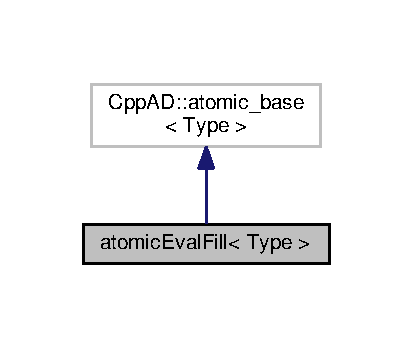
\includegraphics[width=198pt]{classatomicEvalFill__inherit__graph}
\end{center}
\end{figure}


Collaboration diagram for atomic\+Eval\+Fill$<$ Type $>$\+:\nopagebreak
\begin{figure}[H]
\begin{center}
\leavevmode
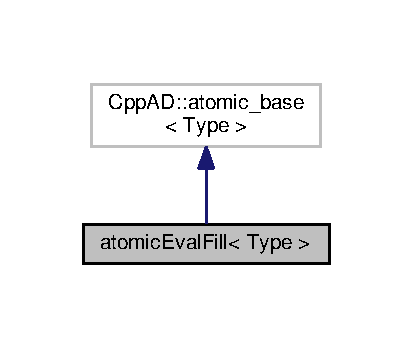
\includegraphics[width=198pt]{classatomicEvalFill__coll__graph}
\end{center}
\end{figure}
\subsubsection*{Public Member Functions}
\begin{DoxyCompactItemize}
\item 
\hypertarget{classatomicEvalFill_af03c332649d669228d335f86981df5b7}{}\hyperlink{classatomicEvalFill_af03c332649d669228d335f86981df5b7}{atomic\+Eval\+Fill} (const char $\ast$name, \hyperlink{classcovafill}{covafill}$<$ A\+D$<$ Type $>$ $>$ cf\+\_\+)\label{classatomicEvalFill_af03c332649d669228d335f86981df5b7}

\begin{DoxyCompactList}\small\item\em Constructs class to evaluate atomic function. \end{DoxyCompactList}\end{DoxyCompactItemize}


\subsubsection{Detailed Description}
\subsubsection*{template$<$class Type$>$class atomic\+Eval\+Fill$<$ Type $>$}

Cpp\+A\+D atomic class to use estimated derivatives in automatic differentiation. See Cpp\+A\+D\+::atomic\+\_\+base for further documentation. 

The documentation for this class was generated from the following file\+:\begin{DoxyCompactItemize}
\item 
atomic.\+hpp\end{DoxyCompactItemize}

\hypertarget{classatomicEvalTree}{}\subsection{atomic\+Eval\+Tree$<$ Type $>$ Class Template Reference}
\label{classatomicEvalTree}\index{atomic\+Eval\+Tree$<$ Type $>$@{atomic\+Eval\+Tree$<$ Type $>$}}


Cpp\+A\+D atomic class to use estimated derivatives in automatic differentiation. See Cpp\+A\+D\+::atomic\+\_\+base for further documentation.  




Inheritance diagram for atomic\+Eval\+Tree$<$ Type $>$\+:\nopagebreak
\begin{figure}[H]
\begin{center}
\leavevmode
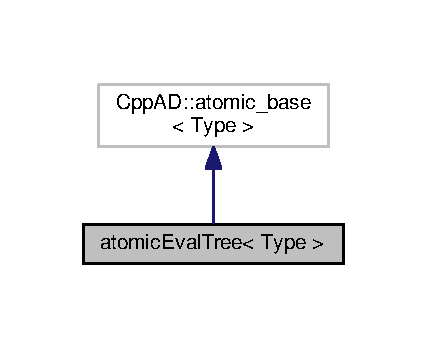
\includegraphics[width=205pt]{classatomicEvalTree__inherit__graph}
\end{center}
\end{figure}


Collaboration diagram for atomic\+Eval\+Tree$<$ Type $>$\+:\nopagebreak
\begin{figure}[H]
\begin{center}
\leavevmode
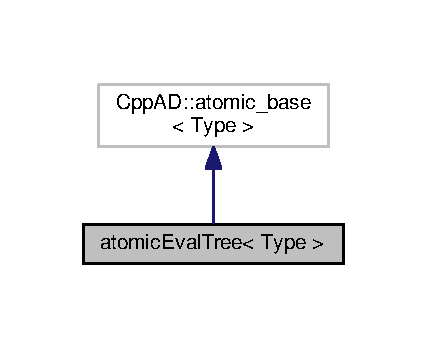
\includegraphics[width=205pt]{classatomicEvalTree__coll__graph}
\end{center}
\end{figure}
\subsubsection*{Public Member Functions}
\begin{DoxyCompactItemize}
\item 
\hypertarget{classatomicEvalTree_a25bf0015d015c8798adea407be763119}{}\hyperlink{classatomicEvalTree_a25bf0015d015c8798adea407be763119}{atomic\+Eval\+Tree} (const char $\ast$name, \hyperlink{classcovatree}{covatree}$<$ A\+D$<$ Type $>$ $>$ ct\+\_\+)\label{classatomicEvalTree_a25bf0015d015c8798adea407be763119}

\begin{DoxyCompactList}\small\item\em Constructs class to evaluate atomic function. \end{DoxyCompactList}\end{DoxyCompactItemize}


\subsubsection{Detailed Description}
\subsubsection*{template$<$class Type$>$class atomic\+Eval\+Tree$<$ Type $>$}

Cpp\+A\+D atomic class to use estimated derivatives in automatic differentiation. See Cpp\+A\+D\+::atomic\+\_\+base for further documentation. 

The documentation for this class was generated from the following file\+:\begin{DoxyCompactItemize}
\item 
atomic\+\_\+\+Tree.\+hpp\end{DoxyCompactItemize}

\hypertarget{classbicubicInterpolation}{}\subsection{bicubic\+Interpolation$<$ scalartype\+\_\+ $>$ Class Template Reference}
\label{classbicubicInterpolation}\index{bicubic\+Interpolation$<$ scalartype\+\_\+ $>$@{bicubic\+Interpolation$<$ scalartype\+\_\+ $>$}}


Class for bi-\/cubic interpolation of local polynomial regression on a square.  




Inheritance diagram for bicubic\+Interpolation$<$ scalartype\+\_\+ $>$\+:\nopagebreak
\begin{figure}[H]
\begin{center}
\leavevmode
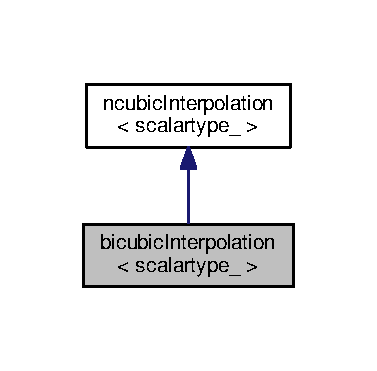
\includegraphics[width=181pt]{classbicubicInterpolation__inherit__graph}
\end{center}
\end{figure}


Collaboration diagram for bicubic\+Interpolation$<$ scalartype\+\_\+ $>$\+:\nopagebreak
\begin{figure}[H]
\begin{center}
\leavevmode
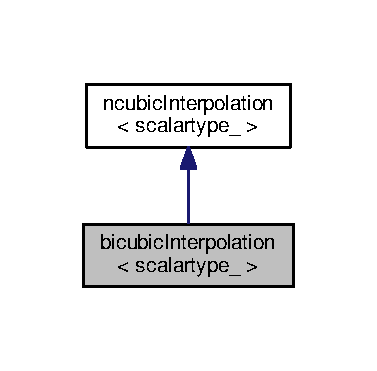
\includegraphics[width=181pt]{classbicubicInterpolation__coll__graph}
\end{center}
\end{figure}
\subsubsection*{Public Member Functions}
\begin{DoxyCompactItemize}
\item 
\hypertarget{classbicubicInterpolation_a1f0aee534884e0679c56ac069218dd71}{}\hyperlink{classbicubicInterpolation_a1f0aee534884e0679c56ac069218dd71}{bicubic\+Interpolation} (\hyperlink{classcovafill}{covafill}$<$ scalartype $>$ $\ast$cf, vectortype \hyperlink{classncubicInterpolation_a5360669149e2182a478f74941c4fb008}{min\+Coord}, vectortype \hyperlink{classncubicInterpolation_a3bd706effb987f94c92f4c89605c7e7c}{max\+Coord})\label{classbicubicInterpolation_a1f0aee534884e0679c56ac069218dd71}

\begin{DoxyCompactList}\small\item\em Constructs a \hyperlink{classbicubicInterpolation}{bicubic\+Interpolation} class from a covafill class {\itshape cf}, an boundaries of the interpolation square defined by the minimum coordinates, {\itshape min\+Coord}, and maximum coordinates, {\itshape max\+Coord}, in each dimension, e.\+g., min\+Coord = (0,0) and max\+Coord = (1,1). \end{DoxyCompactList}\item 
\hypertarget{classbicubicInterpolation_a9b5aab51903b774190b8806f85b65a2a}{}virtual vectortype \hyperlink{classbicubicInterpolation_a9b5aab51903b774190b8806f85b65a2a}{operator()} (vectortype newcoord)\label{classbicubicInterpolation_a9b5aab51903b774190b8806f85b65a2a}

\begin{DoxyCompactList}\small\item\em Calculates the interpolation prediction at {\itshape newcoord}. \end{DoxyCompactList}\end{DoxyCompactItemize}
\subsubsection*{Additional Inherited Members}


\subsubsection{Detailed Description}
\subsubsection*{template$<$typename scalartype\+\_\+$>$class bicubic\+Interpolation$<$ scalartype\+\_\+ $>$}

Class for bi-\/cubic interpolation of local polynomial regression on a square. 

The documentation for this class was generated from the following file\+:\begin{DoxyCompactItemize}
\item 
bicubic\+Interpolation.\+hpp\end{DoxyCompactItemize}

\hypertarget{classcovafill}{}\subsection{covafill$<$ scalartype\+\_\+ $>$ Class Template Reference}
\label{classcovafill}\index{covafill$<$ scalartype\+\_\+ $>$@{covafill$<$ scalartype\+\_\+ $>$}}


Class to do local polynomial regression.  


\subsubsection*{Public Member Functions}
\begin{DoxyCompactItemize}
\item 
\hypertarget{classcovafill_ad04c0d86b0bf096b3a38dd866523643a}{}\hyperlink{classcovafill_ad04c0d86b0bf096b3a38dd866523643a}{covafill} (const \hyperlink{classcovafill}{covafill}$<$ scalartype\+\_\+ $>$ \&x)\label{classcovafill_ad04c0d86b0bf096b3a38dd866523643a}

\begin{DoxyCompactList}\small\item\em Constructs a covafill class from another covafill class {\itshape x}. \end{DoxyCompactList}\item 
\hypertarget{classcovafill_ad270e8490cb357aa42df53e56477d3b0}{}\hyperlink{classcovafill_ad270e8490cb357aa42df53e56477d3b0}{covafill} (matrixtype coordinates\+\_\+, vectortype observations\+\_\+)\label{classcovafill_ad270e8490cb357aa42df53e56477d3b0}

\begin{DoxyCompactList}\small\item\em Constructs a covafill class with coordinates matrix {\itshape coordinates\+\_\+}, observation vector {\itshape obervations}, bandwiths 1, and polynomial degree 2. \end{DoxyCompactList}\item 
\hypertarget{classcovafill_acf5f5cbc366e8626d20872a972922093}{}\hyperlink{classcovafill_acf5f5cbc366e8626d20872a972922093}{covafill} (matrixtype coordinates\+\_\+, vectortype observations\+\_\+, scalartype h\+\_\+, int p\+\_\+)\label{classcovafill_acf5f5cbc366e8626d20872a972922093}

\begin{DoxyCompactList}\small\item\em Constructs a covafill class with coordinates matrix {\itshape coordinates\+\_\+}, observation vector {\itshape obervations}, bandwiths {\itshape h\+\_\+}, and polynomial degree {\itshape p\+\_\+}. \end{DoxyCompactList}\item 
\hypertarget{classcovafill_a7990c15b88e372938b258f9ffe67334e}{}\hyperlink{classcovafill_a7990c15b88e372938b258f9ffe67334e}{covafill} (matrixtype coordinates\+\_\+, vectortype observations\+\_\+, vectortype h\+\_\+, int p\+\_\+)\label{classcovafill_a7990c15b88e372938b258f9ffe67334e}

\begin{DoxyCompactList}\small\item\em Constructs a covafill class with coordinates matrix {\itshape coordinates\+\_\+}, observation vector {\itshape obervations}, bandwiths {\itshape h\+\_\+}, and polynomial degree {\itshape p\+\_\+}. \end{DoxyCompactList}\item 
int \hyperlink{classcovafill_a9fdfc9fb312a1848d2b1258b3a3d56a1}{get\+Dim} () const 
\item 
void \hyperlink{classcovafill_a7be100b5c111aa446578116c119e564b}{set\+H} (scalartype h\+\_\+)
\item 
void \hyperlink{classcovafill_aec6cd784c27dc9692ef25dc5b20fe97b}{set\+H} (vectortype h\+\_\+)
\item 
\hypertarget{classcovafill_abf579279adbd0ff452e00cd91f4ada93}{}vectortype \hyperlink{classcovafill_abf579279adbd0ff452e00cd91f4ada93}{operator()} (vectortype x0, bool return\+All=false) const \label{classcovafill_abf579279adbd0ff452e00cd91f4ada93}

\begin{DoxyCompactList}\small\item\em Calculates the local polynomial regression estimate at {\itshape x0}. If {\itshape return\+All} is false, then only the function and first derivative estimates are returned. Otherwise all estimates are returned. \end{DoxyCompactList}\item 
\hypertarget{classcovafill_a6e76b761e31f54838ef6590e36746d3b}{}vectortype \hyperlink{classcovafill_a6e76b761e31f54838ef6590e36746d3b}{operator()} (vectortype x0, scalartype exclude\+Radius, bool return\+All=false) const \label{classcovafill_a6e76b761e31f54838ef6590e36746d3b}

\begin{DoxyCompactList}\small\item\em Calculates the local polynomial regression estimate at {\itshape x0}. All observations with coordinates $ x $ such that $ \|x-x_0\| > r $, where {\itshape r} is {\itshape exlude\+Radius}. If {\itshape return\+All} is false, then only the function and first derivative estimates are returned. Otherwise all estimates are returned. \end{DoxyCompactList}\item 
\hypertarget{classcovafill_ad7a89edf7a67e8e8994d9a782b476d27}{}\hyperlink{classcovafill}{covafill}$<$ scalartype $>$ \& \hyperlink{classcovafill_ad7a89edf7a67e8e8994d9a782b476d27}{operator=} (const \hyperlink{classcovafill}{covafill}$<$ scalartype $>$ \&rhs)\label{classcovafill_ad7a89edf7a67e8e8994d9a782b476d27}

\begin{DoxyCompactList}\small\item\em Assignment operator for covafill. \end{DoxyCompactList}\end{DoxyCompactItemize}
\subsubsection*{Public Attributes}
\begin{DoxyCompactItemize}
\item 
matrixtype \hyperlink{classcovafill_aafa672d0bd7df22b0524c99dc6978b2d}{coordinates}
\item 
vectortype \hyperlink{classcovafill_a81186c0884235f65e014350579617a74}{observations}
\item 
int \hyperlink{classcovafill_a6aaea280399bd705581e3c387d1f7750}{p}
\item 
vectortype \hyperlink{classcovafill_a60ed2bdd2d36c6cc24e3682006263eaa}{h}
\end{DoxyCompactItemize}


\subsubsection{Detailed Description}
\subsubsection*{template$<$typename scalartype\+\_\+$>$class covafill$<$ scalartype\+\_\+ $>$}

Class to do local polynomial regression. 

\subsubsection{Member Function Documentation}
\hypertarget{classcovafill_a9fdfc9fb312a1848d2b1258b3a3d56a1}{}\index{covafill@{covafill}!get\+Dim@{get\+Dim}}
\index{get\+Dim@{get\+Dim}!covafill@{covafill}}
\paragraph[{get\+Dim}]{\setlength{\rightskip}{0pt plus 5cm}template$<$typename scalartype\+\_\+ $>$ int {\bf covafill}$<$ scalartype\+\_\+ $>$\+::get\+Dim (
\begin{DoxyParamCaption}
{}
\end{DoxyParamCaption}
) const}\label{classcovafill_a9fdfc9fb312a1848d2b1258b3a3d56a1}
Returns the covariate dimension. \hypertarget{classcovafill_a7be100b5c111aa446578116c119e564b}{}\index{covafill@{covafill}!set\+H@{set\+H}}
\index{set\+H@{set\+H}!covafill@{covafill}}
\paragraph[{set\+H}]{\setlength{\rightskip}{0pt plus 5cm}template$<$typename scalartype\+\_\+ $>$ void {\bf covafill}$<$ scalartype\+\_\+ $>$\+::set\+H (
\begin{DoxyParamCaption}
\item[{scalartype}]{h\+\_\+}
\end{DoxyParamCaption}
)}\label{classcovafill_a7be100b5c111aa446578116c119e564b}
Sets all bandwiths to h\+\_\+. 

Referenced by covafill$<$ scalartype\+\_\+ $>$\+::covafill().

\hypertarget{classcovafill_aec6cd784c27dc9692ef25dc5b20fe97b}{}\index{covafill@{covafill}!set\+H@{set\+H}}
\index{set\+H@{set\+H}!covafill@{covafill}}
\paragraph[{set\+H}]{\setlength{\rightskip}{0pt plus 5cm}template$<$typename scalartype\+\_\+ $>$ void {\bf covafill}$<$ scalartype\+\_\+ $>$\+::set\+H (
\begin{DoxyParamCaption}
\item[{vectortype}]{h\+\_\+}
\end{DoxyParamCaption}
)}\label{classcovafill_aec6cd784c27dc9692ef25dc5b20fe97b}
Sets the bandwiths from a vector. The length of h\+\_\+ must match the covariate dimension. 

\subsubsection{Member Data Documentation}
\hypertarget{classcovafill_aafa672d0bd7df22b0524c99dc6978b2d}{}\index{covafill@{covafill}!coordinates@{coordinates}}
\index{coordinates@{coordinates}!covafill@{covafill}}
\paragraph[{coordinates}]{\setlength{\rightskip}{0pt plus 5cm}template$<$typename scalartype\+\_\+$>$ matrixtype {\bf covafill}$<$ scalartype\+\_\+ $>$\+::coordinates}\label{classcovafill_aafa672d0bd7df22b0524c99dc6978b2d}
Coordinates/covariates of input. 

Referenced by covatree$<$ scalartype\+\_\+ $>$\+::covatree(), and covafill$<$ scalartype\+\_\+ $>$\+::operator=().

\hypertarget{classcovafill_a60ed2bdd2d36c6cc24e3682006263eaa}{}\index{covafill@{covafill}!h@{h}}
\index{h@{h}!covafill@{covafill}}
\paragraph[{h}]{\setlength{\rightskip}{0pt plus 5cm}template$<$typename scalartype\+\_\+$>$ vectortype {\bf covafill}$<$ scalartype\+\_\+ $>$\+::h}\label{classcovafill_a60ed2bdd2d36c6cc24e3682006263eaa}
Vector of (positive) bandwiths -\/ one for each covariate. 

Referenced by covafill$<$ scalartype\+\_\+ $>$\+::operator=().

\hypertarget{classcovafill_a81186c0884235f65e014350579617a74}{}\index{covafill@{covafill}!observations@{observations}}
\index{observations@{observations}!covafill@{covafill}}
\paragraph[{observations}]{\setlength{\rightskip}{0pt plus 5cm}template$<$typename scalartype\+\_\+$>$ vectortype {\bf covafill}$<$ scalartype\+\_\+ $>$\+::observations}\label{classcovafill_a81186c0884235f65e014350579617a74}
Input observations. 

Referenced by covafill$<$ scalartype\+\_\+ $>$\+::operator=().

\hypertarget{classcovafill_a6aaea280399bd705581e3c387d1f7750}{}\index{covafill@{covafill}!p@{p}}
\index{p@{p}!covafill@{covafill}}
\paragraph[{p}]{\setlength{\rightskip}{0pt plus 5cm}template$<$typename scalartype\+\_\+$>$ int {\bf covafill}$<$ scalartype\+\_\+ $>$\+::p}\label{classcovafill_a6aaea280399bd705581e3c387d1f7750}
Polynomial degree. 

Referenced by covafill$<$ scalartype\+\_\+ $>$\+::operator=().



The documentation for this class was generated from the following files\+:\begin{DoxyCompactItemize}
\item 
covafill.\+hpp\item 
covafill\+\_\+constructors.\+hpp\item 
covafill\+\_\+operators.\+hpp\item 
covafill\+\_\+private\+Functions.\+hpp\item 
covafill\+\_\+public\+Functions.\+hpp\end{DoxyCompactItemize}

\hypertarget{classjags_1_1covafillJAGS_1_1covafillJAGS}{}\subsection{jags\+:\+:covafill\+J\+A\+G\+S\+:\+:covafill\+J\+A\+G\+S Class Reference}
\label{classjags_1_1covafillJAGS_1_1covafillJAGS}\index{jags\+::covafill\+J\+A\+G\+S\+::covafill\+J\+A\+G\+S@{jags\+::covafill\+J\+A\+G\+S\+::covafill\+J\+A\+G\+S}}


Class that defines the covafill function for local polynomial regression to be used in a J\+A\+G\+S model.  




Inheritance diagram for jags\+:\+:covafill\+J\+A\+G\+S\+:\+:covafill\+J\+A\+G\+S\+:\nopagebreak
\begin{figure}[H]
\begin{center}
\leavevmode
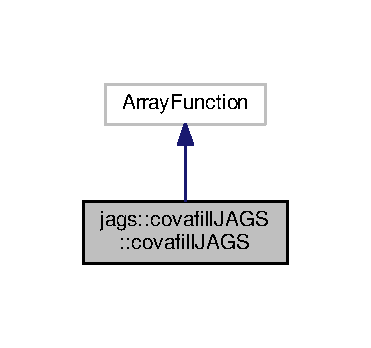
\includegraphics[width=178pt]{classjags_1_1covafillJAGS_1_1covafillJAGS__inherit__graph}
\end{center}
\end{figure}


Collaboration diagram for jags\+:\+:covafill\+J\+A\+G\+S\+:\+:covafill\+J\+A\+G\+S\+:\nopagebreak
\begin{figure}[H]
\begin{center}
\leavevmode
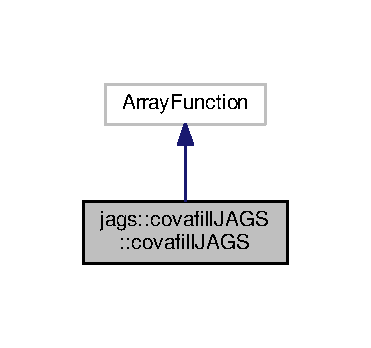
\includegraphics[width=178pt]{classjags_1_1covafillJAGS_1_1covafillJAGS__coll__graph}
\end{center}
\end{figure}
\subsubsection*{Public Member Functions}
\begin{DoxyCompactItemize}
\item 
\hypertarget{classjags_1_1covafillJAGS_1_1covafillJAGS_aaff4734c50b3acdb85a7db82aef92cb7}{}\hyperlink{classjags_1_1covafillJAGS_1_1covafillJAGS_aaff4734c50b3acdb85a7db82aef92cb7}{covafill\+J\+A\+G\+S} ()\label{classjags_1_1covafillJAGS_1_1covafillJAGS_aaff4734c50b3acdb85a7db82aef92cb7}

\begin{DoxyCompactList}\small\item\em Default constructor. \end{DoxyCompactList}\item 
\hypertarget{classjags_1_1covafillJAGS_1_1covafillJAGS_adf1dc88d47a4bb95fe3ff5f0f340bb9c}{}void \hyperlink{classjags_1_1covafillJAGS_1_1covafillJAGS_adf1dc88d47a4bb95fe3ff5f0f340bb9c}{evaluate} (double $\ast$value, std\+::vector$<$ double const $\ast$ $>$ const \&args, std\+::vector$<$ std\+::vector$<$ unsigned int $>$ $>$ const \&dims) const \label{classjags_1_1covafillJAGS_1_1covafillJAGS_adf1dc88d47a4bb95fe3ff5f0f340bb9c}

\begin{DoxyCompactList}\small\item\em Evaluates a covafill object. \end{DoxyCompactList}\item 
\hypertarget{classjags_1_1covafillJAGS_1_1covafillJAGS_aaaa1d047cb8bba343c665bd48b4b8b2b}{}std\+::vector$<$ unsigned int $>$ \hyperlink{classjags_1_1covafillJAGS_1_1covafillJAGS_aaaa1d047cb8bba343c665bd48b4b8b2b}{dim} (std\+::vector$<$ std\+::vector$<$ unsigned int $>$ $>$ const \&dims, std\+::vector$<$ double const $\ast$ $>$ const \&values) const \label{classjags_1_1covafillJAGS_1_1covafillJAGS_aaaa1d047cb8bba343c665bd48b4b8b2b}

\begin{DoxyCompactList}\small\item\em Returns dimension of result. \end{DoxyCompactList}\item 
\hypertarget{classjags_1_1covafillJAGS_1_1covafillJAGS_a76aaca437c8bd6cbd0f315ab00f03ac8}{}bool \hyperlink{classjags_1_1covafillJAGS_1_1covafillJAGS_a76aaca437c8bd6cbd0f315ab00f03ac8}{check\+Parameter\+Dim} (std\+::vector$<$ std\+::vector$<$ unsigned int $>$ $>$ const \&dims) const \label{classjags_1_1covafillJAGS_1_1covafillJAGS_a76aaca437c8bd6cbd0f315ab00f03ac8}

\begin{DoxyCompactList}\small\item\em Function to check parameter dimensions. Currently returns true for any input dimension. \end{DoxyCompactList}\end{DoxyCompactItemize}


\subsubsection{Detailed Description}
Class that defines the covafill function for local polynomial regression to be used in a J\+A\+G\+S model. 

The documentation for this class was generated from the following files\+:\begin{DoxyCompactItemize}
\item 
covafill\+J\+A\+G\+S.\+hpp\item 
covafill\+J\+A\+G\+S.\+cpp\end{DoxyCompactItemize}

\hypertarget{classjags_1_1covafillJAGS_1_1covafillModule}{}\subsection{jags\+:\+:covafill\+J\+A\+G\+S\+:\+:covafill\+Module Class Reference}
\label{classjags_1_1covafillJAGS_1_1covafillModule}\index{jags\+::covafill\+J\+A\+G\+S\+::covafill\+Module@{jags\+::covafill\+J\+A\+G\+S\+::covafill\+Module}}


Class that defines a J\+A\+G\+S Module for local polynomial regression.  




Inheritance diagram for jags\+:\+:covafill\+J\+A\+G\+S\+:\+:covafill\+Module\+:\nopagebreak
\begin{figure}[H]
\begin{center}
\leavevmode
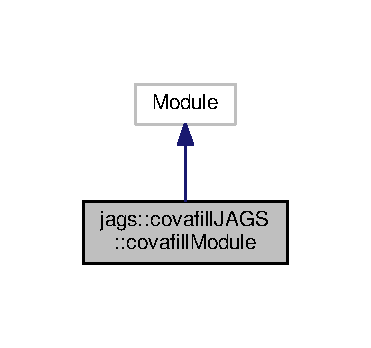
\includegraphics[width=178pt]{classjags_1_1covafillJAGS_1_1covafillModule__inherit__graph}
\end{center}
\end{figure}


Collaboration diagram for jags\+:\+:covafill\+J\+A\+G\+S\+:\+:covafill\+Module\+:\nopagebreak
\begin{figure}[H]
\begin{center}
\leavevmode
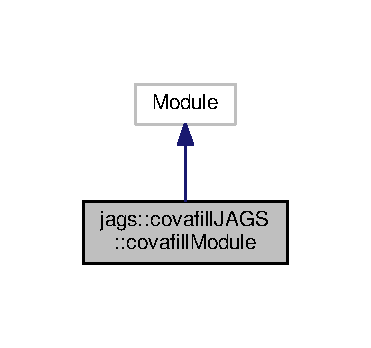
\includegraphics[width=178pt]{classjags_1_1covafillJAGS_1_1covafillModule__coll__graph}
\end{center}
\end{figure}


\subsubsection{Detailed Description}
Class that defines a J\+A\+G\+S Module for local polynomial regression. 

The documentation for this class was generated from the following file\+:\begin{DoxyCompactItemize}
\item 
covafill.\+cpp\end{DoxyCompactItemize}

\hypertarget{classcovanode}{}\subsection{covanode$<$ scalartype\+\_\+ $>$ Class Template Reference}
\label{classcovanode}\index{covanode$<$ scalartype\+\_\+ $>$@{covanode$<$ scalartype\+\_\+ $>$}}


Class that defines nodes of a covatree.  


\subsubsection*{Public Member Functions}
\begin{DoxyCompactItemize}
\item 
\hyperlink{classcovanode_aeb9afb3b2447653b72a1fafdeb5eed00}{covanode} (matrixtype coord\+Split, scalartype min\+Split\+Size\+\_\+, \hyperlink{classcovafill}{covafill}$<$ scalartype $>$ $\ast$cf, vectortype min\+Coords, vectortype max\+Coords)
\begin{DoxyCompactList}\small\item\em Constructs a node in a covatree. \end{DoxyCompactList}\item 
\hypertarget{classcovanode_a9eec5ac7fa598d7d855e0433111d396a}{}int \hyperlink{classcovanode_a9eec5ac7fa598d7d855e0433111d396a}{get\+Dim} ()\label{classcovanode_a9eec5ac7fa598d7d855e0433111d396a}

\begin{DoxyCompactList}\small\item\em Get coordinate dimension. \end{DoxyCompactList}\item 
\hypertarget{classcovanode_a6e4ccc5051d2b52192a8cc70a0a401bb}{}vectortype \hyperlink{classcovanode_a6e4ccc5051d2b52192a8cc70a0a401bb}{operator()} (vectortype newcoord)\label{classcovanode_a6e4ccc5051d2b52192a8cc70a0a401bb}

\begin{DoxyCompactList}\small\item\em Returns the interpolated value at {\itshape newcoord} of the local polynomial regressions at the corners of the boundary box. \end{DoxyCompactList}\end{DoxyCompactItemize}


\subsubsection{Detailed Description}
\subsubsection*{template$<$typename scalartype\+\_\+$>$class covanode$<$ scalartype\+\_\+ $>$}

Class that defines nodes of a covatree. 

\subsubsection{Constructor \& Destructor Documentation}
\hypertarget{classcovanode_aeb9afb3b2447653b72a1fafdeb5eed00}{}\index{covanode@{covanode}!covanode@{covanode}}
\index{covanode@{covanode}!covanode@{covanode}}
\paragraph[{covanode}]{\setlength{\rightskip}{0pt plus 5cm}template$<$typename scalartype\+\_\+ $>$ {\bf covanode}$<$ scalartype\+\_\+ $>$\+::{\bf covanode} (
\begin{DoxyParamCaption}
\item[{matrixtype}]{coord\+Split, }
\item[{scalartype}]{min\+Split\+Size\+\_\+, }
\item[{{\bf covafill}$<$ scalartype $>$ $\ast$}]{cf, }
\item[{vectortype}]{min\+Coords, }
\item[{vectortype}]{max\+Coords}
\end{DoxyParamCaption}
)}\label{classcovanode_aeb9afb3b2447653b72a1fafdeb5eed00}


Constructs a node in a covatree. 


\begin{DoxyParams}{Parameters}
{\em coord\+Split} & The remaining coordinates in the split at which we are now creating a note \\
\hline
{\em min\+Split\+Size\+\_\+} & The minimum number of coordinates at which the node will create a subtree. \\
\hline
{\em cf} & A covafill object for local polynomial regression at the corners of the boundary box. \\
\hline
{\em min\+Coords} & Minimum coordinates of the boundary box corners, e.\+g., (0,0) in two dimensions. \\
\hline
{\em max\+Coords} & Maximum coordinates of the boundary box corners, e.\+g., (1,1) in two dimensions. \\
\hline
\end{DoxyParams}


The documentation for this class was generated from the following files\+:\begin{DoxyCompactItemize}
\item 
covanode.\+hpp\item 
covanode\+\_\+constructors.\+hpp\item 
covanode\+\_\+operators.\+hpp\end{DoxyCompactItemize}

\hypertarget{classcovatree}{}\subsection{covatree$<$ scalartype\+\_\+ $>$ Class Template Reference}
\label{classcovatree}\index{covatree$<$ scalartype\+\_\+ $>$@{covatree$<$ scalartype\+\_\+ $>$}}


Class that defines a covatree for search tree approximated local polynomial regression.  


\subsubsection*{Public Member Functions}
\begin{DoxyCompactItemize}
\item 
\hypertarget{classcovatree_af2e211e962e7c21cdf55dd2c9c87ed17}{}\hyperlink{classcovatree_af2e211e962e7c21cdf55dd2c9c87ed17}{covatree} (scalartype min\+Split\+Size\+\_\+, \hyperlink{classcovafill}{covafill}$<$ scalartype $>$ $\ast$cf)\label{classcovatree_af2e211e962e7c21cdf55dd2c9c87ed17}

\begin{DoxyCompactList}\small\item\em Constructs a tree from a covafill object {\itshape cf} with minimum number of coordinates at which a sub tree will be created {\itshape min\+Split\+Size\+\_\+}. \end{DoxyCompactList}\item 
\hypertarget{classcovatree_a3bc91d5b1516c0ac0b4c9f02e871ef06}{}int \hyperlink{classcovatree_a3bc91d5b1516c0ac0b4c9f02e871ef06}{get\+Dim} ()\label{classcovatree_a3bc91d5b1516c0ac0b4c9f02e871ef06}

\begin{DoxyCompactList}\small\item\em Get coordinate dimension. \end{DoxyCompactList}\item 
\hypertarget{classcovatree_a2fd5facb6a97d7356428ef07141c6481}{}vectortype \hyperlink{classcovatree_a2fd5facb6a97d7356428ef07141c6481}{operator()} (vectortype newcoord) const \label{classcovatree_a2fd5facb6a97d7356428ef07141c6481}

\begin{DoxyCompactList}\small\item\em Returns the interpolated value at {\itshape newcoord} of the local polynomial regressions at the corners of the boundary box. \end{DoxyCompactList}\end{DoxyCompactItemize}


\subsubsection{Detailed Description}
\subsubsection*{template$<$typename scalartype\+\_\+$>$class covatree$<$ scalartype\+\_\+ $>$}

Class that defines a covatree for search tree approximated local polynomial regression. 

The documentation for this class was generated from the following files\+:\begin{DoxyCompactItemize}
\item 
covatree.\+hpp\item 
covatree\+\_\+constructors.\+hpp\end{DoxyCompactItemize}

\hypertarget{classcubicInterpolation}{}\subsection{cubic\+Interpolation$<$ scalartype\+\_\+ $>$ Class Template Reference}
\label{classcubicInterpolation}\index{cubic\+Interpolation$<$ scalartype\+\_\+ $>$@{cubic\+Interpolation$<$ scalartype\+\_\+ $>$}}


Class for cubic interpolation in dimension 1-\/3 of local polynomial regression on a square.  


\subsubsection*{Public Member Functions}
\begin{DoxyCompactItemize}
\item 
\hypertarget{classcubicInterpolation_a315eb8b62c04985416cd0e9fd7655022}{}\hyperlink{classcubicInterpolation_a315eb8b62c04985416cd0e9fd7655022}{cubic\+Interpolation} (\hyperlink{classcovafill}{covafill}$<$ scalartype $>$ $\ast$cf, vectortype min\+Coords, vectortype max\+Coords)\label{classcubicInterpolation_a315eb8b62c04985416cd0e9fd7655022}

\begin{DoxyCompactList}\small\item\em Constructs a \hyperlink{classbicubicInterpolation}{bicubic\+Interpolation} class from a covafill class {\itshape cf}, an boundaries of the interpolation square defined by the minimum coordinates, {\itshape min\+Coord}, and maximum coordinates, {\itshape max\+Coord}, in each dimension, e.\+g., min\+Coord = (0,0) and max\+Coord = (1,1). \end{DoxyCompactList}\item 
\hypertarget{classcubicInterpolation_ac566e2bd2ece485f7e63689316045e59}{}vectortype \hyperlink{classcubicInterpolation_ac566e2bd2ece485f7e63689316045e59}{operator()} (vectortype newcoord)\label{classcubicInterpolation_ac566e2bd2ece485f7e63689316045e59}

\begin{DoxyCompactList}\small\item\em Returns the interpolation prediction at {\itshape newcoord}. \end{DoxyCompactList}\end{DoxyCompactItemize}


\subsubsection{Detailed Description}
\subsubsection*{template$<$typename scalartype\+\_\+$>$class cubic\+Interpolation$<$ scalartype\+\_\+ $>$}

Class for cubic interpolation in dimension 1-\/3 of local polynomial regression on a square. 

The documentation for this class was generated from the following file\+:\begin{DoxyCompactItemize}
\item 
cubic\+Interpolation.\+hpp\end{DoxyCompactItemize}

\hypertarget{classncubicInterpolation}{}\subsection{ncubic\+Interpolation$<$ scalartype\+\_\+ $>$ Class Template Reference}
\label{classncubicInterpolation}\index{ncubic\+Interpolation$<$ scalartype\+\_\+ $>$@{ncubic\+Interpolation$<$ scalartype\+\_\+ $>$}}


Class for n-\/cubic interpolation (n = 1,2,3) of local polynomial regression on a square. The class should not be used as anything but a common parent for the dimension specific interpolation classes.  




Inheritance diagram for ncubic\+Interpolation$<$ scalartype\+\_\+ $>$\+:\nopagebreak
\begin{figure}[H]
\begin{center}
\leavevmode
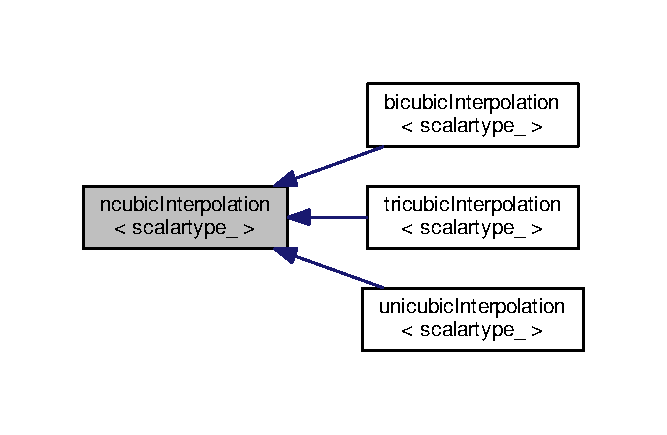
\includegraphics[width=320pt]{classncubicInterpolation__inherit__graph}
\end{center}
\end{figure}
\subsubsection*{Public Member Functions}
\begin{DoxyCompactItemize}
\item 
\hypertarget{classncubicInterpolation_aefd7ad3e2a5582ac0c4556b71c1b0cc9}{}\hyperlink{classncubicInterpolation_aefd7ad3e2a5582ac0c4556b71c1b0cc9}{ncubic\+Interpolation} (\hyperlink{classcovafill}{covafill}$<$ scalartype $>$ $\ast$cf, vectortype min\+Coord\+\_\+, vectortype max\+Coord\+\_\+)\label{classncubicInterpolation_aefd7ad3e2a5582ac0c4556b71c1b0cc9}

\begin{DoxyCompactList}\small\item\em Constructs a n-\/cubic\+Interpolation class from a covafill class {\itshape cf}, an boundaries of the interpolation square defined by the minimum coordinates, {\itshape min\+Coord}, and maximum coordinates, {\itshape max\+Coord}, in each dimension, e.\+g., min\+Coord = (0,0) and max\+Coord = (1,1). \end{DoxyCompactList}\item 
\hypertarget{classncubicInterpolation_a83cfa933656a532951dcdd97ef7f50f1}{}virtual vectortype \hyperlink{classncubicInterpolation_a83cfa933656a532951dcdd97ef7f50f1}{operator()} (vectortype newcoord)=0\label{classncubicInterpolation_a83cfa933656a532951dcdd97ef7f50f1}

\begin{DoxyCompactList}\small\item\em Calculates the interpolation prediction at {\itshape newcoord}. \end{DoxyCompactList}\end{DoxyCompactItemize}
\subsubsection*{Protected Member Functions}
\begin{DoxyCompactItemize}
\item 
\hypertarget{classncubicInterpolation_adf4741f9535abf6ff6e232b0aa818b46}{}\hyperlink{classncubicInterpolation_adf4741f9535abf6ff6e232b0aa818b46}{ncubic\+Interpolation} (vectortype min\+Coord\+\_\+, vectortype max\+Coord\+\_\+)\label{classncubicInterpolation_adf4741f9535abf6ff6e232b0aa818b46}

\begin{DoxyCompactList}\small\item\em Constructor from coordinates. Should in general not be called. \end{DoxyCompactList}\end{DoxyCompactItemize}
\subsubsection*{Protected Attributes}
\begin{DoxyCompactItemize}
\item 
int \hyperlink{classncubicInterpolation_ab0be3a8f99377893bf23724c3e3e4f18}{dim}
\item 
vectortype \hyperlink{classncubicInterpolation_a5360669149e2182a478f74941c4fb008}{min\+Coord}
\item 
vectortype \hyperlink{classncubicInterpolation_a3bd706effb987f94c92f4c89605c7e7c}{max\+Coord}
\end{DoxyCompactItemize}


\subsubsection{Detailed Description}
\subsubsection*{template$<$typename scalartype\+\_\+$>$class ncubic\+Interpolation$<$ scalartype\+\_\+ $>$}

Class for n-\/cubic interpolation (n = 1,2,3) of local polynomial regression on a square. The class should not be used as anything but a common parent for the dimension specific interpolation classes. 

\subsubsection{Member Data Documentation}
\hypertarget{classncubicInterpolation_ab0be3a8f99377893bf23724c3e3e4f18}{}\index{ncubic\+Interpolation@{ncubic\+Interpolation}!dim@{dim}}
\index{dim@{dim}!ncubic\+Interpolation@{ncubic\+Interpolation}}
\paragraph[{dim}]{\setlength{\rightskip}{0pt plus 5cm}template$<$typename scalartype\+\_\+$>$ int {\bf ncubic\+Interpolation}$<$ scalartype\+\_\+ $>$\+::dim\hspace{0.3cm}{\ttfamily [protected]}}\label{classncubicInterpolation_ab0be3a8f99377893bf23724c3e3e4f18}
Dimension of coordinates, i.\+e., the n in n-\/cubic. \hypertarget{classncubicInterpolation_a3bd706effb987f94c92f4c89605c7e7c}{}\index{ncubic\+Interpolation@{ncubic\+Interpolation}!max\+Coord@{max\+Coord}}
\index{max\+Coord@{max\+Coord}!ncubic\+Interpolation@{ncubic\+Interpolation}}
\paragraph[{max\+Coord}]{\setlength{\rightskip}{0pt plus 5cm}template$<$typename scalartype\+\_\+$>$ vectortype {\bf ncubic\+Interpolation}$<$ scalartype\+\_\+ $>$\+::max\+Coord\hspace{0.3cm}{\ttfamily [protected]}}\label{classncubicInterpolation_a3bd706effb987f94c92f4c89605c7e7c}
maximum coordinates of boundary box. \hypertarget{classncubicInterpolation_a5360669149e2182a478f74941c4fb008}{}\index{ncubic\+Interpolation@{ncubic\+Interpolation}!min\+Coord@{min\+Coord}}
\index{min\+Coord@{min\+Coord}!ncubic\+Interpolation@{ncubic\+Interpolation}}
\paragraph[{min\+Coord}]{\setlength{\rightskip}{0pt plus 5cm}template$<$typename scalartype\+\_\+$>$ vectortype {\bf ncubic\+Interpolation}$<$ scalartype\+\_\+ $>$\+::min\+Coord\hspace{0.3cm}{\ttfamily [protected]}}\label{classncubicInterpolation_a5360669149e2182a478f74941c4fb008}
Minimum coordinates of boundary box. 

The documentation for this class was generated from the following file\+:\begin{DoxyCompactItemize}
\item 
ncubic\+Interpolation.\+hpp\end{DoxyCompactItemize}

\hypertarget{classtricubicInterpolation}{}\subsection{tricubic\+Interpolation$<$ scalartype\+\_\+ $>$ Class Template Reference}
\label{classtricubicInterpolation}\index{tricubic\+Interpolation$<$ scalartype\+\_\+ $>$@{tricubic\+Interpolation$<$ scalartype\+\_\+ $>$}}


Class for tri-\/cubic interpolation of local polynomial regression on a square.  




Inheritance diagram for tricubic\+Interpolation$<$ scalartype\+\_\+ $>$\+:\nopagebreak
\begin{figure}[H]
\begin{center}
\leavevmode
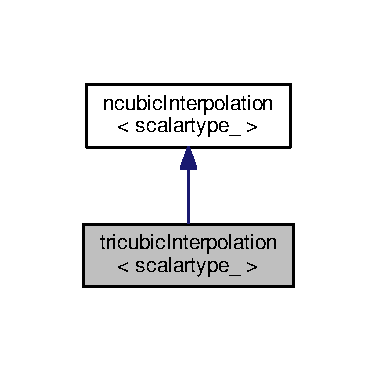
\includegraphics[width=181pt]{classtricubicInterpolation__inherit__graph}
\end{center}
\end{figure}


Collaboration diagram for tricubic\+Interpolation$<$ scalartype\+\_\+ $>$\+:\nopagebreak
\begin{figure}[H]
\begin{center}
\leavevmode
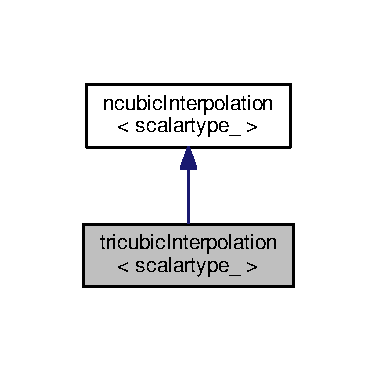
\includegraphics[width=181pt]{classtricubicInterpolation__coll__graph}
\end{center}
\end{figure}
\subsubsection*{Public Member Functions}
\begin{DoxyCompactItemize}
\item 
\hypertarget{classtricubicInterpolation_ad5e9cb968974cea893a884a7f0420111}{}\hyperlink{classtricubicInterpolation_ad5e9cb968974cea893a884a7f0420111}{tricubic\+Interpolation} (\hyperlink{classcovafill}{covafill}$<$ scalartype $>$ $\ast$cf, vectortype \hyperlink{classncubicInterpolation_a5360669149e2182a478f74941c4fb008}{min\+Coord}, vectortype \hyperlink{classncubicInterpolation_a3bd706effb987f94c92f4c89605c7e7c}{max\+Coord})\label{classtricubicInterpolation_ad5e9cb968974cea893a884a7f0420111}

\begin{DoxyCompactList}\small\item\em Constructs a \hyperlink{classtricubicInterpolation}{tricubic\+Interpolation} class from a covafill class {\itshape cf}, an boundaries of the interpolation square defined by the minimum coordinates, {\itshape min\+Coord}, and maximum coordinates, {\itshape max\+Coord}, in each dimension, e.\+g., min\+Coord = (0,0,0) and max\+Coord = (1,1,1). \end{DoxyCompactList}\item 
\hypertarget{classtricubicInterpolation_a8554c02565bafd34a90e3af5350e1e59}{}virtual vectortype \hyperlink{classtricubicInterpolation_a8554c02565bafd34a90e3af5350e1e59}{operator()} (vectortype newcoord)\label{classtricubicInterpolation_a8554c02565bafd34a90e3af5350e1e59}

\begin{DoxyCompactList}\small\item\em Calculates the interpolation prediction at {\itshape newcoord}. \end{DoxyCompactList}\end{DoxyCompactItemize}
\subsubsection*{Additional Inherited Members}


\subsubsection{Detailed Description}
\subsubsection*{template$<$typename scalartype\+\_\+$>$class tricubic\+Interpolation$<$ scalartype\+\_\+ $>$}

Class for tri-\/cubic interpolation of local polynomial regression on a square. 

The documentation for this class was generated from the following file\+:\begin{DoxyCompactItemize}
\item 
tricubic\+Interpolation.\+hpp\end{DoxyCompactItemize}

\hypertarget{classunicubicInterpolation}{}\subsection{unicubic\+Interpolation$<$ scalartype\+\_\+ $>$ Class Template Reference}
\label{classunicubicInterpolation}\index{unicubic\+Interpolation$<$ scalartype\+\_\+ $>$@{unicubic\+Interpolation$<$ scalartype\+\_\+ $>$}}


Class for cubic interpolation of local polynomial regression on a square.  




Inheritance diagram for unicubic\+Interpolation$<$ scalartype\+\_\+ $>$\+:\nopagebreak
\begin{figure}[H]
\begin{center}
\leavevmode
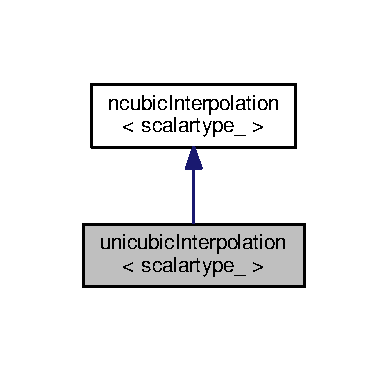
\includegraphics[width=186pt]{classunicubicInterpolation__inherit__graph}
\end{center}
\end{figure}


Collaboration diagram for unicubic\+Interpolation$<$ scalartype\+\_\+ $>$\+:\nopagebreak
\begin{figure}[H]
\begin{center}
\leavevmode
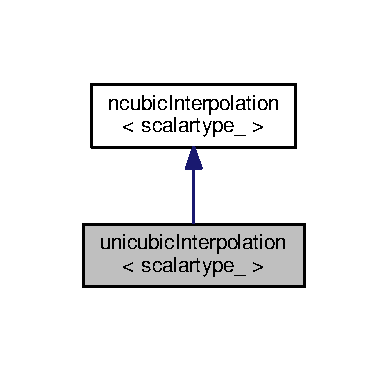
\includegraphics[width=186pt]{classunicubicInterpolation__coll__graph}
\end{center}
\end{figure}
\subsubsection*{Public Member Functions}
\begin{DoxyCompactItemize}
\item 
\hypertarget{classunicubicInterpolation_ac693f198959412ec4ad42a6a7ceba4c0}{}\hyperlink{classunicubicInterpolation_ac693f198959412ec4ad42a6a7ceba4c0}{unicubic\+Interpolation} (\hyperlink{classcovafill}{covafill}$<$ scalartype $>$ $\ast$cf, vectortype \hyperlink{classncubicInterpolation_a5360669149e2182a478f74941c4fb008}{min\+Coord}, vectortype \hyperlink{classncubicInterpolation_a3bd706effb987f94c92f4c89605c7e7c}{max\+Coord})\label{classunicubicInterpolation_ac693f198959412ec4ad42a6a7ceba4c0}

\begin{DoxyCompactList}\small\item\em Constructs a \hyperlink{classunicubicInterpolation}{unicubic\+Interpolation} class from a covafill class {\itshape cf}, an boundaries of the interpolation square defined by the minimum coordinates, {\itshape min\+Coord}, and maximum coordinates, {\itshape max\+Coord}, in each dimension, e.\+g., min\+Coord = 0 and max\+Coord = 1. \end{DoxyCompactList}\item 
\hypertarget{classunicubicInterpolation_a9a385ca116d23bf0280dd12cc3887ac4}{}virtual vectortype \hyperlink{classunicubicInterpolation_a9a385ca116d23bf0280dd12cc3887ac4}{operator()} (vectortype newcoord)\label{classunicubicInterpolation_a9a385ca116d23bf0280dd12cc3887ac4}

\begin{DoxyCompactList}\small\item\em Calculates the interpolation prediction at {\itshape newcoord}. \end{DoxyCompactList}\end{DoxyCompactItemize}
\subsubsection*{Additional Inherited Members}


\subsubsection{Detailed Description}
\subsubsection*{template$<$typename scalartype\+\_\+$>$class unicubic\+Interpolation$<$ scalartype\+\_\+ $>$}

Class for cubic interpolation of local polynomial regression on a square. 

The documentation for this class was generated from the following file\+:\begin{DoxyCompactItemize}
\item 
unicubic\+Interpolation.\+hpp\end{DoxyCompactItemize}

%--- End generated contents ---

% Index
\newpage
\phantomsection
\clearemptydoublepage
\addcontentsline{toc}{section}{Index}
\printindex

\end{document}
